\chapter{Preliminaries}\label{chapter:intro}
\section{Introduction}\label{sec:intro}

This collection is the published manuscript of the \textit{Navajo Corpus of Historical Narratives} (NCHN) (\cite{Denk:2025zp}). The NCHN is a digital compilation of 9 annotated narratives chosen from the \textit{Navajo Historical Selections} published by Robert W. Young and William Morgan in the 1950s. The \textit{Navajo Historical Selections}, in turn, are texts selected from the monthly newspaper \textit{Ádahooníłígíí} written in the Navajo language (\textit{Diné Bizaad}) and published in the Southwestern United States from 1943 to 1957 (\cite[51]{McCarty:2002bz}) and translated by Young and Morgan.

Compared to the wealth of texts available for Navajo relative to other Native American languages, this collection represents only a small fraction. While the Navajo Corpus for Historical Narratives (NCHN) was primarily developed to create a repository of morphologically annotated words and to establish a consistent glossing strategy for Navajo, to enhance both educational resources and linguistic conventions (see \cite{Denk:2024aq}), it also offers critical insights into the complex history encompassing the struggle for land reclamation and the integration of traditional narratives. This selection reflects the diversity of Navajo thought of the late 19th and first half of the 20th century and invites both linguistic and cultural investigation, expanding the pool of materials for a Diné philology.

The corpus text presented here contains three versions of the story ``The trouble at Round Rock'', published in \citet{Young:1952cy}; the latest edition is from 2015. These narratives depict a pivotal event in Diné history: the fight between the chief, Black Horse, and Navajo Agent Shipley in October 1892, after Navajos had moved back to their homeland from their forced exile in Fort Sumner. This fight was a reaction to new government policies imposed whereby children ought to be relocated from their families and placed in English boarding schools. This story is told from three different Navajo perspectives, one of the narrators witnessing the event directly. The remaining 6 annotated texts originate from the 25 narratives published in the Historical Collections by the same authors two years later (\cite{Young:1954jz}) and provide diverse personal, political, historical, and traditional accounts of Navajo life. With over 10,000 words, the NCHN is the largest morphologically annotated collection of Navajo texts, and we are pleased to present it as part of the Open Text Collection series.

\section{The setting}

Navajo speakers refer to themselves as ``Diné'' which means ``The People.'' The traditional homeland of the Diné, known as Diné Bikéyah, encompasses the region between the Four Sacred Mountains in the Southwestern United States: \textit{Sisnaajiní} or Blanca Peak in the east, \textit{Tsoodził} or Mt. Taylor in the south; \textit{Dok’o’oosłííd} or the San Francisco Peaks in the west; and \textit{Dibéntsaa} or Hesperus Peak in the north.  These form the spiritual and historical foundation of the Navajo world (\cite{Iverson:2002it}; \cite{Blake:2001oe}; \cite{Linford:2000hb}; \cite{Griffin-Pierce:1997aq}). According to Navajo oral history, these mountains not only delineate the boundaries of their homeland but are key symbols of their cosmology and cultural identity (\cite{Blake:2001oe}).

The Navajo Nation is the largest Native American reservation in the US, covering parts of Arizona, New Mexico, and Utah. It is characterized by its vast arid landscape, stretching across approximately 27,000 square miles. Major towns like Window Rock (\textit{Tségháhoodzání}; the capital), Kayenta (\textit{Tó Dínéeshzheeʼ}), and Shiprock (\textit{Tsé Bitʼaʼí}) serve as cultural and economic centers, while smaller towns with chapter houses are scattered throughout the region, including traditional settlements like family-owned sheep camps and \textit{hooghan} dwellings.

The relationship between the Diné and their land is strong and predates colonization, but subsequent, modern events have also contributed to the awareness of what it means to be Navajo. In 1863, the Navajo Long Walk -- a forced relocation imposed on the Navajo people -- left a lasting impact on the bond of future generations with their homeland. This devastating event, marked by military defeat and captivity, has since become a central element of modern Navajo identity (\cite{Csordas:2000ft}). This experience disrupted their way of life and following the return to their homeland and the establishment of the Navajo reservation by the treaty of 1868, the Long Walk still persists in the collective mind of Diné people and informs the interpretation of the historical events that happened thereafter (\cite{Csordas:2000ft}). However, the long walk was not the only event that would bring hardship to the people. After the reservation was established, Navajos were still forced to assimilate into white society. With the opening of Bureau of Indian Affairs across the reservation, the US government displaced children from their family environment by sending them to boarding schools, where they would be taught in an English-only environment and children who would speak their own language would be punished. Understandably, Navajo families were suspicious of or outright against this implementation, setting the conditions for fights between agents and Navajo leaders. One of these fights, the trouble at Round Rock, is presented here in three narratives.

In the following decades, the US government continued its attempts of forced assimilation, for example through the Livestock Reduction act during the Great Depression. The act consisted of reducing animals with the pretense that large herds would compromise agricultural yields and lead to further erosion of areas affected by the Dust Bowl. Navajos overwhelmingly opposed the act as undermining their very existence and way of life but weren't able to revoke it. This tragedy is recorded in the historical selection by featuring two Navajo voices (Our Abuse; The Special Grazing Regulation).

Despite this and following exploitative practices like Uranium mining and fracking, the historical, geographic and traditional knowledge remains unbroken. And part of this knowledge can be seen in additional narratives that depict traditional stories which have remained in the common consciousness since time immemorial. The relationship between Navajos and their homeland is therefore not only characterized by the negative effects endured during colonization, but by the enduring traditional knowledge, inside and outside the reservation, and new avenues of creativity. Part of this strong connection is probably due to their close family relationships that are frequently brought to consciousness when introducing one another, namely the clan system. 

In Navajo society, every individual belongs to four clans, two inherited from the mother and two from the father, following a matrilineal system. The clans are associated with geographical areas and some of them are featured in the creation stories. Clan affiliation also influences marriage patterns, as it is forbidden to marry within one's own maternal or paternal clan. In this way, Navajos maintain a system of exogamy that fosters social unity across different kinship groups. Some traditional stories and rituals are also considered the property of specific clans, passed down through generations as part of the oral tradition. Women play a central role as guardians of these traditions (\cite{McCloskey:2007mb}; \cite{Denetdale:2015vo}).
    
According to the 2019 census as reported by Ethnologue (\cite{ethnologue2021}), there are approximately 300,000 ethnic Navajos, of whom 170,000 are speakers. \citet{Denetclaw:2017sd} further reported 7,600 monolinguals. Despite having the largest number of speakers among indigenous languages in the U.S., it is classified as ``threatened'' (6b in the Ethnologue EGIDS scale), indicating that speaker numbers have declined since this census and continue to decrease. Navajo is taught in schools on the reservation, and various language revitalization programs have been developed to address concerns about language attrition. Bilingualism is a defining feature in Diné society due to Navajo being spoken in school and integrated in school curricula alongside English. Despite this, Navajo exhibits a relatively small number of loans (According to Wiktionary, 58 English and 38 Spanish loans)\footnote{\url{https://en.wiktionary.org/wiki/Category:Navajo_borrowed_terms}}. While their language was unrelated to the ones of Pueblo tribes in the area (Keresan, Tanoan, Zuñi, Hopi), Navajo communities were culturally connected to them through trade and intermarriage before European colonization (\cite{Warburton:2005le}). Despite the high levels of English fluency today, many Diné, even in urban environments, remain deeply committed to maintaining their culture and connection to the ancestral land between the Four Sacred Mountains.

\section{Grammar sketch} 

\subsection{Introduction}

Navajo is a Southern Athabaskan (or Apachean) language, part of the larger Athabaskan language family, which extends across Canada, Alaska, and the southwestern United States. \textit{Athabaskan} was chosen by Albert Gallatin in 1863 referring to the Lake Athabasca where these languages are spoken (\cite[17]{Gallatin:1836ph}). The name itself originates from the Moose Cree word \textit{Āðapāskāw} ``[where] there are plants one after the other'', describing the lake (\cite[52]{Bright:2004kl}). The alternative denomination for the family is \textit{Dene}, reflecting the common word for `people' across these language, which is also present in \textit{Diné Bizaad}, the endonym for Navajo. Navajo is spoken primarily within the Navajo Nation, but generally in the territory spanning parts of Arizona, New Mexico, and Utah, and Colorado.

Like Athabaskan languages, Navajo is a coronal-heavy language with multiple contrasts in stops and affricates. Syntactically, Navajo is known for a tendency for subject-object-verb order (or: Agent, Patient, Verb), although the order of constituents is rather determined by animacy and topicality (\cite{Willie:2000up}). Navajo is a head-final and head-marking language in which participants precede the verbs that index them, possessor nouns precede possessed nouns that index them, noun phrases precede postpositions that index them. Subordinate clauses tend to precede main clauses, linked by enclitics attached to them.

Morphologically, Navajo is heavily prefixing, and features enclitics. While noun words have little morphology, verbs feature a great array of prefixes. The verbal structure is commonly divided into multiple morpheme positions which are grouped into three domains: disjunct (outer prefixes; positions 0-III), conjunct (inner prefixes; positions IV-IX) and stem (or root, position X). The difference between conjunct and disjunct prefixes is mainly phonological (\cite{Sapir:1967pj}; \cite{Kari:1973jy,Kari:1975tg}; and \cite{Young:1987uj}, \cite{McDonough:1995hp}). Each domain hosts lexical (or thematic), inflectional and derivational information sketched in \tabref{tab:navverb}.

\begin{table}
\caption{Domains of the Navajo verb and their morphological categories}
\label{tab:navverb}
\begin{tabularx}{\textwidth}{QQQ}
    \lsptoprule
    \textsc{disjunct domain}&\textsc{conjunct domain}&\textsc{stem domain}\\
    \midrule
    Lexical information, (Lexical) Aspect&Lexical information, (Lexical) Aspect&Lexical information, (Lexical) Aspect\\
    \tablevspace
    Derivation, Agreement&Derivation, Valence, Tense \& Mood&Tense \& Mood, Agreement (Number)\\
    \tablevspace
    &Agreement&\\
    \lspbottomrule
\end{tabularx}
\end{table}

Navajo features multiple conjugations, in which morphemes from all these domains interact. The distributed nature of these morpheme categories and the fused and syncretic forms of paradigms makes Navajo and other Athapaskan languages quite difficult to segment and analyze.

In the following sections, we will provide a larger overview of its phonology, morphology, and syntax, and emphasize its most typologically striking features. To understand the glossing convention that we adopted for the NCHN and for this publication, we will provide a sketch of different morphological analyses that will allow us to justify the choice in the segmentation of verbs.

\subsection{Phonology}

The following phonological review will concentrate on the phonemic inventory of consonants and vowels.

\subsubsection{Consonants}

Navajo has a primarily obstruent, coronal-heavy inventory. This inventory is shared by all Athabaskan languages. These obstruents contain stops, fricatives, affricates, with their laryngeal realizations as plain, ejective, and aspirated. In addition, Navajo has a lateral series involving lateral fricatives and affricates. Athabaskan languages exhibit a series of aspirated stops. However, in Navajo, the stops /t\textsuperscript{h}/ and /k\textsuperscript{h}/ are not realized as aspiration in the laryngeal sense (open glottis after stop release). Rather, these stops are coarticulated with a heavily spirantized velar release (\cite{McDonough:2008gh}; \cite{Iskarous:2012qz}) and are therefore interpreted as /tx/ and /kx/ phonemes. This is a feature across Athabaskan languages, as witnessed in Northern Athabaskan languages spoken along the Mackenzie River (\textit{Dene Speech Atlas}, \cite{McDonough:2013fk}). \tabref{tab:consonants} shows the organization of Navajo consonants using IPA and orthographic symbols.

\begin{sidewaystable}
\caption{Consonant inventory of Navajo. Each cell represents a contrastive phoneme. The orthographic symbols used in \citet{Young:1987uj} are in angle brackets.}
\label{tab:consonants}
\fittable{
\begin{tabular}{llc cccc ccc c}
    \lsptoprule
    && \multicolumn{1}{c}{\textsc{labial}} & \multicolumn{4}{c}{\textsc{coronal}} & \multicolumn{3}{c}{\textsc{palato-velar}}&\textsc{glottal}\\
    \cmidrule(lr){4-7}\cmidrule(lr){8-10}
        &&\multicolumn{1}{c}{}& \textsc{plain} & \textsc{anterior} & \textsc{posterior} & \textsc{lateral}&\textsc{palatal}&\textsc{velar}&\textsc{labio-}\textsc{velar}&\\
    \midrule
    \multirow{10}{*}{\rotatebox[origin=l]{90}{\textsc{occlusives}\phantom{aa}}}&\multirow{2}{*}{\textsc{nasal}}&\multicolumn{1}{c}{m}&n&&&&&&&\\
    &&\multicolumn{1}{c}{⟨m⟩}&⟨n⟩&&&&&&&\\
    &\multirow{2}{*}{\textsc{plain}}&\multicolumn{1}{c}{p}&t&ts&tʃ&t\textsuperscript{l}&&k&&ʔ\\
    &&\multicolumn{1}{c}{⟨b⟩}&⟨d⟩&⟨dz⟩&⟨j⟩&⟨dl⟩&&⟨g⟩&&⟨'⟩\\
    &\multirow{2}{*}{\textsc{glottalized}}&\multicolumn{1}{l}{}&t'& ts'& tʃ'& tɬ'&&k’&&\\
    &&\multicolumn{1}{l}{}&⟨t'⟩&⟨ts'⟩&⟨ch'⟩& ⟨tł'⟩&&⟨k’⟩&&\\
    &\multirow{2}{*}{\textsc{aspirated}}&\multicolumn{1}{l}{}&& ts\textsuperscript{h}& tʃ\textsuperscript{h}&tɬ\textsuperscript{h}&&&&\\
    &&\multicolumn{1}{l}{}&&⟨ts⟩&⟨ch⟩&⟨tł⟩&&&&\\
    &\multirow{2}{*}{\textsc{velar fric.}}&\multicolumn{1}{l}{}& tx&&&&& kx&kx\textsuperscript{w}&\\
    &&\multicolumn{1}{l}{}&⟨t⟩&&&&&⟨k⟩&⟨kw⟩&\\
    \midrule
    \multirow{6}{*}{\rotatebox[origin=l]{90}{\textsc{continuants}\phantom{a}}}&\multirow{2}{*}{\textsc{voiceless}}&&&s&ʃ&ɬ&&x&x\textsuperscript{w}&h\\
    &&&&⟨s⟩&⟨sh⟩&⟨ł⟩&&⟨h, x⟩&⟨hw⟩&⟨h⟩\\    
    &\multirow{2}{*}{\textsc{voiced}}&&&z&ʒ&&&ɣ&ɣ\textsuperscript{w}&\\
    &&&&⟨z⟩&⟨zh⟩&&&⟨gh⟩&⟨w⟩&\\
    &\multirow{2}{*}{\textsc{approximant}}&&&&&l&j&&&\\
    &&&&&&⟨l⟩&⟨y⟩&&&\\
    \lspbottomrule
\end{tabular}
}
\end{sidewaystable}

\tabref{tab:consonants} combines analyses from \citet{Young:1987uj} and \citet{McDonough:2003tp} but uses additional labels to condense the information. Among these are the stops with a complex release: \textit{anterior}, \textit{posterior}\footnote{This is justified also by the phonological process of consonant harmony, which is captured in a [±anterior] contrast in \citet[50--51]{McDonough:2003tp}.} and \textit{lateral}, referring to alveolar, postalveolar, and lateral fricative components. This series is extended to the continuants further down, where the manner of articulation of the onset is the same as the manner of the release (fricatives and approximants). The table does not include allophones. A notable allophonic rule is palatalization (\cite[vx]{Young:1987uj}) which applies to coronals and velars. It is worth mentioning that \citet[4]{McDonough:2003tp} lists /ç/ as part of the inventory, but \citet[vx]{Young:1987uj} treat it as an allophone of /x/. In addition, the distinction between fricatives and approximants is not always clear-cut. This is because the approximant /j/ has a fricative allophone [ʝ] and /ɣʷ/ and /ɣ/ have approximant allophones [w] and [ɰ]. For more information on the allophonic rules, consult \citet[xii-xv]{Young:1987uj}, \citet{McDonough:2003tp}; further analyses on allophones are \citet{Iskarous:2012qz}, \citet{McDonough:1990gn}, \citet{Palakurthy:2019pw}, and earlier accounts such as \citet{Saville:1968tm} and \citet{Harris:1945to}. 

Most importantly, the full set of phonological contrasts listed in \tabref{tab:consonants} is attested only in stem onsets. As \citet[7]{McDonough:2003tp} observes, this highly restricted phonemic distribution renders the traditional notion of a phonemic inventory somewhat misleading, since the contrasts are confined to a single positional slot within a multisyllabic word. This restriction is particularly evident in the aspirated and glottalized stop series (\cite[43--45]{McDonough:2003tp}). These are characterized by a relatively long release phase. In these segments, the interval between the stop closure and voice onset is substantially longer than in their plain counterparts (/p/, /t/, /ts/, /tʃ/, /tl/). On the basis of this durational property, \citet[81]{McDonough:2003tp} classifies these segments as ``complex,'' distinguishing them from the plain stops and affricates but also from consonant clusters that would rather be constrained by syllable structure (cf. \cite[75]{McDonough:2003tp}). Outside of stems, the consonants that occur are ``almost exclusively coronal'' (\cite[43]{McDonough:2003tp}). \citet{McDonough:2008gh} demonstrate that this simplex-complex contrast among consonants is likely a cross-Athabaskan characteristic.

\subsubsection{Vowels}

There are four different vowel qualities (/a/, /e/, /i/, /o/). The vowels contrast in length, tone (high, low) and nasality, resulting in 16 vowel contrasts. There is a quality difference between the long and short high front [ɪ] vs. [i:] (\cite[xii]{Young:1987uj}). The vowel inventory is presented in \tabref{tab:vowels}.

\begin{table}
\caption{Vowels (monophthongs only, IPA and Navajo orthography in brackets)}
\label{tab:vowels}
\begin{tabularx}{\textwidth}{lQlQl}
    \lsptoprule
    &\multicolumn{2}{c}{\textsc{oral}}~~~~&\multicolumn{2}{c}{\textsc{nasal}}~~~~\\
    \cmidrule(lr){2-3}\cmidrule(lr){4-5}
    &\textsc{short}&\textsc{long}&\textsc{short}&\textsc{long}\\
    \midrule
    \multirow{2}{*}{\textsc{low tone}}&ɑ ɛ ɪ o&ɑː eː iː oː&{ɑ̃} {ɛ̃} {ɪ̃} {õ}&{ɑ̃}ː {ẽ}ː {ĩ}ː {õ}ː\\
    &⟨a, e, i, o⟩&⟨aa, ee, ii, oo⟩&⟨ą, ę, į, ǫ⟩&⟨ąą, ęę, įį, ǫǫ⟩\\
    &&&&\\
    \multirow{2}{*}{\textsc{high tone}}&{ɑ́} {ɛ́} {ɪ́} {ó}&{ɑ́}ː {é}ː {í}ː {ó}ː&{ɑ̃́} {ɛ̃́} {ɪ̃́} {ṍ}&{ɑ̃́}ː {ẽ́}ː {ĩ́}ː {ṍ}ː\\
    &⟨á, é, í, ó⟩&⟨áá, éé, íí, óó⟩&⟨ą́, ę́, į́, ǫ́⟩&⟨ą́ą́, ę́ę́, į́į́, ǫ́ǫ́⟩\\

    \lspbottomrule
\end{tabularx}
\end{table}

Besides the monophthongs, the following diphthongs and vowel clusters exist (according to \cite[xii]{Young:1987uj}): ⟨ai, aii, ąi, ei, eii, ao, oi, oii⟩. Long vowels and diphthongs may exhibit high and low tones successively; this tonal combination is referred to as \textit{rising} and \textit{falling} tones, such as ⟨ę́ę⟩ or ⟨ooí⟩ (\cite[xiii]{Young:1987uj}). However, these falling and rising tones aren't contrastive, as they are always conditioned by morpho-phonological processes such as lengthening, contractions, and assimilation caused by enclitics (same page). For further information on the tonal system and its realization, across Athabaskan, we recommend the reader to consult \citet{Young:1987uj}, \citet{Krauss:2005oq}, \citet{Kingston:2005ef}, \citet{McDonough:2003tp}. The next section discusses the orthographic conventions used for Navajo.

\subsubsection{Orthographic conventions}

The development of Navajo orthography has been a gradual process, influenced by early transcription attempts and evolving into a system that captures Navajo phonetics with increasing precision. Initial recordings by non-Navajo figures like Pedro Bautista Pino, James Hervey Simpson, and J.H. Eaton in the 19th century used English-based transcriptions that approximated, but did not accurately capture, Navajo sounds. A breakthrough came with Washington Matthews in the 1880s, who introduced phonetic symbols like ł, the barred or ``slash-l'' (\cite[53]{Williams:2009om}). This work was further advanced in the early 20th century by Fray Berard Haile and Franciscan missionaries. In 1916, the American Anthropological Association set phonetic standards that influenced Navajo orthography, particularly nasalized vowel representations like the 
``hook'' or ``ogonek'' \ ̨\ (ą, ę, į, ǫ), although digraphs (e.g., ch, dl, ts) were not consistently adopted afterwards (\cite[624]{Herzog:1934hs}).

A major step in standardizing Navajo orthography came in 1943 when Robert Young and William Morgan, under the Office of Indian Affairs, created an accessible, typewriter-compatible alphabet that aligned with the English QWERTY keyboard. This system, initially introduced in \textit{The Navaho Language: The Elements of Navaho Grammar} (\cite{Young:1969qt}), and later refined in their 1980 dictionary (\cite{Young:1980xm}), became the primary writing system for Navajo. The Young and Morgan orthography has since remained the most widely accepted and used system and became a foundational tool for Navajo literacy and linguistic research. The orthographic symbols of this standard are presented in the respective tables for the consonants (\tabref{tab:consonants}) and vowels (\tabref{tab:vowels}).

\subsection{Morphology}

As mentioned in \sectref{sec:intro}, Navajo is heavily prefixing like other Athapaskan languages and features enclitics. Suffixes or proclitics are rare. The distribution of morphological operations is skewed toward the verbs, as this part of speech has most of the prefixes of the language. In contrast, nouns and postpositions exhibit minimal inflection, limited to (possessive) person prefixes and marginal plurality markers, some of which can be interpreted as suffixes; e.g., \textit{'ashkii} `boy' \textit{'ashii-ké} `boys'. Enclitics are numerous, and can be classified into subordinating, relativizing, interrogative, postpositional and adjectival enclitics (\cite[part I:17--23]{Young:1987uj}) attaching to phrases and clauses. Furthermore, because nouns, adverbs, and postpositions are frequently derived from verbs through enclitics, they inherit their complex morphological structure.

Due to its verbal morphological complexity, Navajo and other Athapaskan languages are often considered polysynthetic (\cite{Mithun:1983te, Mithun:2015ta}; \cite{Fortescue:2007sv}, \cite{Sapir:1921bp}), most notably because its verbs ``can function as complete predications in themselves'' (\cite[38]{Mithun:2015ta}). However, this classification is not unanimous. \citet{Mattissen:2004go} notes that Athapaskan languages, including Navajo, are not prototypically polysynthetic (Navajo fulfills only 2 out of 5 criteria). De Reuse (\citeyear{de-Reuse:2009ij}) goes further, rejecting the label for Athapaskan languages on the grounds that they lack ``productive noninflectional concatenation'' (\citeyear[21--22]{de-Reuse:2009ij}). Indeed, some derivational prefixes are highly lexicalized and unproductive, while inflectional categories are interspersed between them, a pattern that has been named ``interrupted synthesis'' (\cite{Kari:1989ja}; \cite{Whorf:1956jt}).

This structure has crucial implications for morphological theory. On the one hand, one can segment verbs into morphs and assign a single meaning to them. On the other hand, one can treat different morphs in the verb as forming a unitary category, a category that is distributed across different elements in the verb.

Example (\ref{exex}) illustrates the verb \textit{nikidadii'níísh} (`We all start to work') using two analytical approaches: linear and distributional.

\ea \label{exex}
    Linear (surface and templatic) and distributional analyses of the verb \textit{nikidadii’níísh} `We all are starting to work' (\cite[634--635]{Young:1987uj})
	\ea \label{exsurf}
        \textit{nikidadii'níísh}\\
        \gll \textup{niki}- \textup{da}- \textup{d}- \textup{[ii’-]} \textup{níísh}\\
        \textsc{th}- \textsc{distr}- \textsc{inc}- [1.\textsc{du}/\textsc{pl}.\textsc{yi}.\textsc{zero}.\textsc{impf}] work.\textsc{mom}.\textsc{impf}\\
		\glt `We all start to work.'
	\ex \label{extempl}
        \textit{nikidadii'níísh}\\
        \glll \textup{niki}- \textup{da}- \textup{di}- \textup{[yi}- \textup{Ø}- \textup{ii}- \textup{d-]} \textup{níísh}\\
		start- \textsc{distr}- \textsc{inc}- [\textsc{trnsl}- \textsc{impf}- 1.\textsc{du}/\textsc{pl}- \textsc{val}-] work.\textsc{mom}.\textsc{impf}\\
        Ib(2) III VIa [VIc VII VIII IX] X\\
		\glt `We all start to work.'
    \ex \label{exdistrs}
        \textit{nikidadii'níísh}\\
        \gll\textup{[niki}\textup{+}\textup{d}\textup{+}\textup{ii’}\textup{+}\textup{níísh]} \textup{[da+ii’]}	\textup{[níísh]}\\
        [Transitional.Inception] [1.\textsc{pl}] [work.\textsc{mom}.\textsc{impf}]\\
		\glt `We all start to work.'
    \z
\z

Linear analyses segment the verb sequentially, assigning each part a distinct function. This can be done on the surface level (\ref{exsurf}) or through a more detailed templatic analysis (\ref{extempl}). A surface-level approach would segment the morphs linearly and assign each morph the features that it expresses. This leads to some morphs exhibiting many grammatical categories, such as \textit{ii'-} `1.\textsc{du}/\textsc{pl}.\textsc{yi}.\textsc{zero}.\textsc{impf}'.

The templatic approach in (\ref{extempl}) is another linear analysis but further decomposes surface-fusional morphs into underlying components, where \textit{ii'-} is analyzed as the combination of the prefixes \textit{yi-Ø-ii-d-} from positions VIc, VII, VIII, and IX, respectively.

A distributional analysis (\ref{exdistrs}), by contrast, groups often non-adjacent morphs into functional categories, such as ``Transitional Inception'' or ``1.\textsc{pl}'', even when a single morph contributes to multiple categories (e.g., \textit{ii'-}). Many linguists prefer this type of analysis for Athabaskan languages in general, and analyze different verb theme categories (\cite{Slate:1989kg}; \cite{Kari:1989ja}; \cite{Hardy:1979jc}), where derivational and inflectional features are properties of the whole verb rather than of individual morphemes.

Navajo morphology can thus be viewed as fusional (one morph, many categories, e.g., 1.\textsc{du}/\textsc{pl}.\textsc{yi}.\textsc{zero}.\textsc{impf}), agglutinative (one morph, one category, e.g., \textit{yi-Ø-ii-d-}) or non-concatenative/distributional (several morphs, one category). This multiplicity of perspectives is reflected in the standard reference (\cite{Young:1987uj, Young:1992bd}), which uses both templatic positions and (fusional) conjugation charts for each verb. We will outline this template and the dictionary's presentation of inflected forms. In addition, we will provide insights from the bipartite approach by \citet{McDonough:1990gn}. These perspectives are essential for understanding the glossing conventions used in the narratives in \sectref{sec:conventions}.

\subsubsection{The verbal template}

\citet{Young:1987uj} and \citet{Young:1992bd} make use of a verbal template that abstracts over fully inflected verb forms by identifying a sequence of morphological positions within the verb. The template serves as an orienting framework that allows readers to locate types of morphemes relative to the order they appear in verbs and to compare Navajo verbal structure with that of other Athabaskan languages. It is not, however, intended as a word-formation mechanism. The template, based on \citet{Young:1987uj} and \citet{Young:1992bd}\footnote{The template was first formulated in the 1987 volume, but the 1992 template provides extra distinctions within positions which are important to explain the glossing conventions. We will therefore use the template from the 1992 version.}, is presented in Table 4 and identifies a sequence of morphological positions, including the stem, subject and object agreement, aspectual and modal marking, valence (classifier), and various derivational or thematic elements.

\begin{xltabular}{\textwidth}{lccX}
    \caption{Summary of the verbal template from \citet[846--854]{Young:1992bd}. Information highlighted in white is considered inflectional; information in grey is considered lexical/thematic/derivational.}\label{tab:verbtemplate}\\
    
    \lsptoprule
        \textsc{position}&\multicolumn{2}{l}{\textsc{sub-}}&\textsc{morphemic category}\\
        &\multicolumn{2}{l}{\textsc{position}}&\\
    \midrule
    \endfirsthead

    \multicolumn{4}{c}%
    {\tablename\ \thetable{} -- continued from previous page}\\
    \lsptoprule
        \textsc{position}&\multicolumn{2}{l}{\textsc{sub-}}&\textsc{morphemic category}\\
        &\multicolumn{2}{l}{\textsc{position}}&\\
    \midrule
    \endhead

    \hline \multicolumn{4}{r}{{Continued on next page}}\\
    \endfoot
    \endlastfoot 
    
        \multirow{2}{*}{0}&&&Object of postposition, Possessor of an incorporated noun (see Position IV for morphemes)\\\hline
        \cellcolor[gray]{.95}&\multirow{3}{*}{a}&&Null Postposition (pronominal prefixes without an incorporated postposition) (see Position IV for morphemes)\\\cline{2-4}
        \rowcolor[gray]{.95}&&1&Postpositional (incorporated postposition)\\\cline{3-4}
        \rowcolor[gray]{.95}&&2&Adverbial-thematic\\\cline{3-4}
        \rowcolor[gray]{.95}&\multirow{-3}{*}{b}&3&Nominal (incorporated noun)\\\cline{2-4}
        \rowcolor[gray]{.95}&c&&Reflexive\\\cline{2-4}
        \rowcolor[gray]{.95}&d&&Reversionary\\\cline{2-4}
        \rowcolor[gray]{.95}\multirow{-9}{*}{I}&e&&Semeliterative\\\hline
        \multirow{2}{*}{II}&&&Iterative\\
        &&&\textit{ná-} \textsc{iter}\\\hline
        \multirow{2}{*}{III}&&&Distributive Plural\\
        &&&\textit{da-} \textsc{distr}\\\hline
        \multirow{11}{*}{IV}&&&Direct object pronouns\\
        &&&\textit{shi-} 1.\textsc{sg}\\
        &&&\textit{ni-} 2.\textsc{sg}\\
        &&&\textit{bi-} 3.\textsc{bi}\\
        &&&\textit{yi-} 3.\textsc{yi}\\
        &&&\textit{ha-} 3.\textsc{anim}\\
        &&&\textit{di-} \textsc{refl}\\
        &&&\textit{’ahi-} \textsc{rec}\\
        &&&\textit{’a-} \textsc{ind}\\
        &&&\textit{nihi-} 1.\textsc{du}/\textsc{pl}\\
        &&&\textit{nihi-} 2.\textsc{du}/\textsc{pl}\\\hline
        \multirow{5}{*}{V}&&&(deictic) Subject third person Pronouns\\
        &&&\textit{ji-} \textsc{anim}\\
        &&&\textit{ho-} \textsc{ar}\\
        &&&\textit{’a-} \textsc{ind}\\
        &&&\textit{’di-} \textsc{agt}.\textsc{pas}\\\hline
        \rowcolor[gray]{.95}&\multirow{2}{*}{a}&&Adverbial-thematic (mostly \textit{di-} morphs), incl. \textit{di- }inceptive and \textit{di-} future; and other morphs\\\cline{2-4}
        \rowcolor[gray]{.95}&\multirow{2}{*}{b}&&Adverbial-thematic (mostly \textit{ni-} morphs), incl. \textit{ni-} terminative\\\cline{2-4}
        \rowcolor[gray]{.95}\multirow{-4}{*}{VI}&\multirow{2}{*}{c}&&Adverbial-thematic (mostly \textit{yi-} morphs), incl. \textit{yi-} transitional/semelfactive\\\hline
        \multirow{6}{*}{VII}&&&Modal-conjugation markers signaling aspect and mood, lexically restricted)\\
        &&&\textit{Ø-} \textsc{impf}/\textsc{perf}/\textsc{usit}\\
        &&&\textit{yi-} \textsc{prog}/\textsc{impf}\\
        &&&\textit{ni-} \textsc{impf}/\textsc{perf}\\
        &&&\textit{si-} \textsc{impf}/\textsc{perf}\\
        &&&\textit{wó-} \textsc{opt}\\\hline
        \multirow{7}{*}{VIII}&&&Verb-incorporated subject pronouns\\
        &&&\textit{sh}- 1.\textsc{sg}\\
        &&&\textit{ni}- 2.\textsc{sg}\\
        &&&\textit{Ø}- 3 (third person, all numbers)\\
        &&&\textit{ii(d)}- 1.\textsc{du}/\textsc{pl}\\
        &&&\textit{oh}- 2.\textsc{du}/\textsc{pl}\\\hline
        \rowcolor[gray]{.95}IX&&&Classifiers\footnotemark \ (these are valence indicators): \textit{Ø}-, \textit{ł}-, \textit{l}-, \textit{d}-\\\hline
        \rowcolor[gray]{.95}\multirow{2}{*}{X}&&&Stem (with different derivational and inflectional alternations)\\
    \lspbottomrule
\end{xltabular}
\footnotetext{The name ``classifier'' is regarded as a misnomer by various Athabaskanists; it is rather a valency indicator (\cite{Kibrik:1996mf}).}

(\ref{ex:intro1}) shows an additional example of how a verb would be glossed following the template, with the number of positions as an additional line:

\ea\label{ex:intro1}
    \textup{Templatic glossing of \textit{ninááshizhneestą́ą́’} (NCHN: CT:2.12)}\\
    \textit{ninááshizhneestą́ą́’}\\
    \gllll \textup{na-} \textup{náá-} \textup{shi-} \textup{zh-} \textup{n-} \textup{ees-} {} {} \textup{tą́ą́’}\\
    \textup{na-} \textup{náá-} \textup{shi-} \textup{ji-} \textup{ni-} \textup{si-} \textup{Ø-} \textup{Ø-} \textup{tą́ą́’}\\
    Ib- Ie- IV- V- VI- VII- VIII- IX- X\\
	\textsc{cont}- \textsc{sitr}- 1.\textsc{sg}- \textsc{anim}- \textsc{th}- \textsc{si}.\textsc{perf}- 3- \textsc{val}- teach.\textsc{cont}.\textsc{perf}\\
    \glt `He has been teaching me again.' \exsource{Text F: \ref{ex:text6-2-12}}
\z

Yet again, one can see that the templatic approach works well for morphs at the left edge of verbs, but conjunct morphs like \textit{ees-} cannot be assigned to a single templatic position. Instead, \textit{ees-} is part of a paradigm that Young and Morgan reference with multiple verb entries. The next section explains how these verb entries are structured.

\subsubsection{Verbal entries in \textit{The Navajo language} (1987)}

In \textit{The Navajo language} (\citeyear{Young:1987uj}), verbs are alphabetized by their first letter as they appear, with each entry headed by a first-person singular imperfective form, e.g., \textit{’ádísk’ąąs} `I am stretching myself'. This verbal entry is shown in \figref{fig:dictexample}.

\begin{figure}
    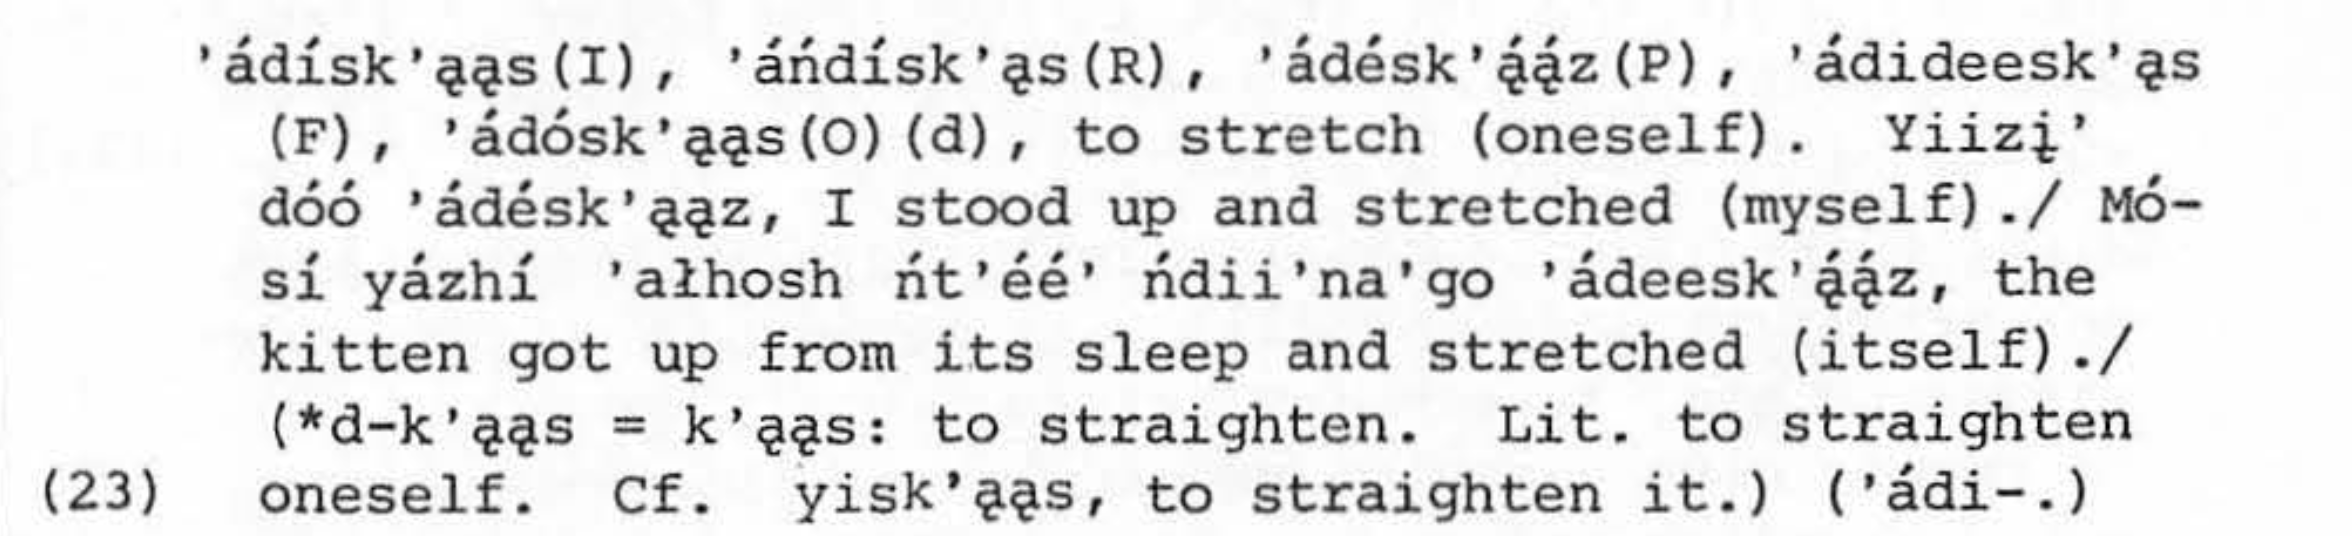
\includegraphics[width=\linewidth]{figures/adiskqqs.png}
    \caption{Example of a verbal entry in the \citet[22]{Young:1987uj} dictionary.}
    \label{fig:dictexample}
\end{figure}

The structure of the verb entry provides the following key information:

\begin{enumerate}
    \item \textbf{Mode forms}: First-person singular forms for the Imperfective (I), Iterative (R), Perfective (P), Future (F), and Optative (O).
    \item \textbf{Classifier}: The valence marker (Position IX) in parentheses (e.g. ``\textbf{\textit{d}}'').
    \item \textbf{Translation}: An English infinitive (e.g., `to stretch (oneself)').
    \item \textbf{Examples}: Illustrative sentences in Navajo translated into English.
    \item \textbf{Stem information}: The classifier-stem shape (e.g., \textbf{\textit{k’ąąs}}, derived from \textbf{\textit{d-k’ąąs}}), which determines stem shape across modes.
    \item \textbf{Stem translation:} The meaning of the stem-classifier combination (e.g., `to straighten').
    \item \textbf{Prefix string and conjugation:} The pre-stem complex (inflectional, derivational, and thematic prefixes) for each mode, either listed directly or referenced to paradigmatic tables (e.g. \textbf{\textit{’ádi-}}, with reference to pg. 23).
    \item \textbf{Derivational links}: References to similar derived verbs (e.g., \textbf{\textit{yisk’ąąs}} `to straighten it').
\end{enumerate}

This organization allows any inflected form to be traced systematically to its stem and conjugation pattern. For example, in the entry for \textit{’ádísk’ąąs} (see \figref{fig:dictexample}), the pre-stem element \textit{’ádi-} is identified as a reflexive prefix. As mentioned above, the entry also indexes a page containing a conjugation table for all verbs sharing this prefix string (see \figref{fig:conjug}).

\begin{figure}
    \centering
    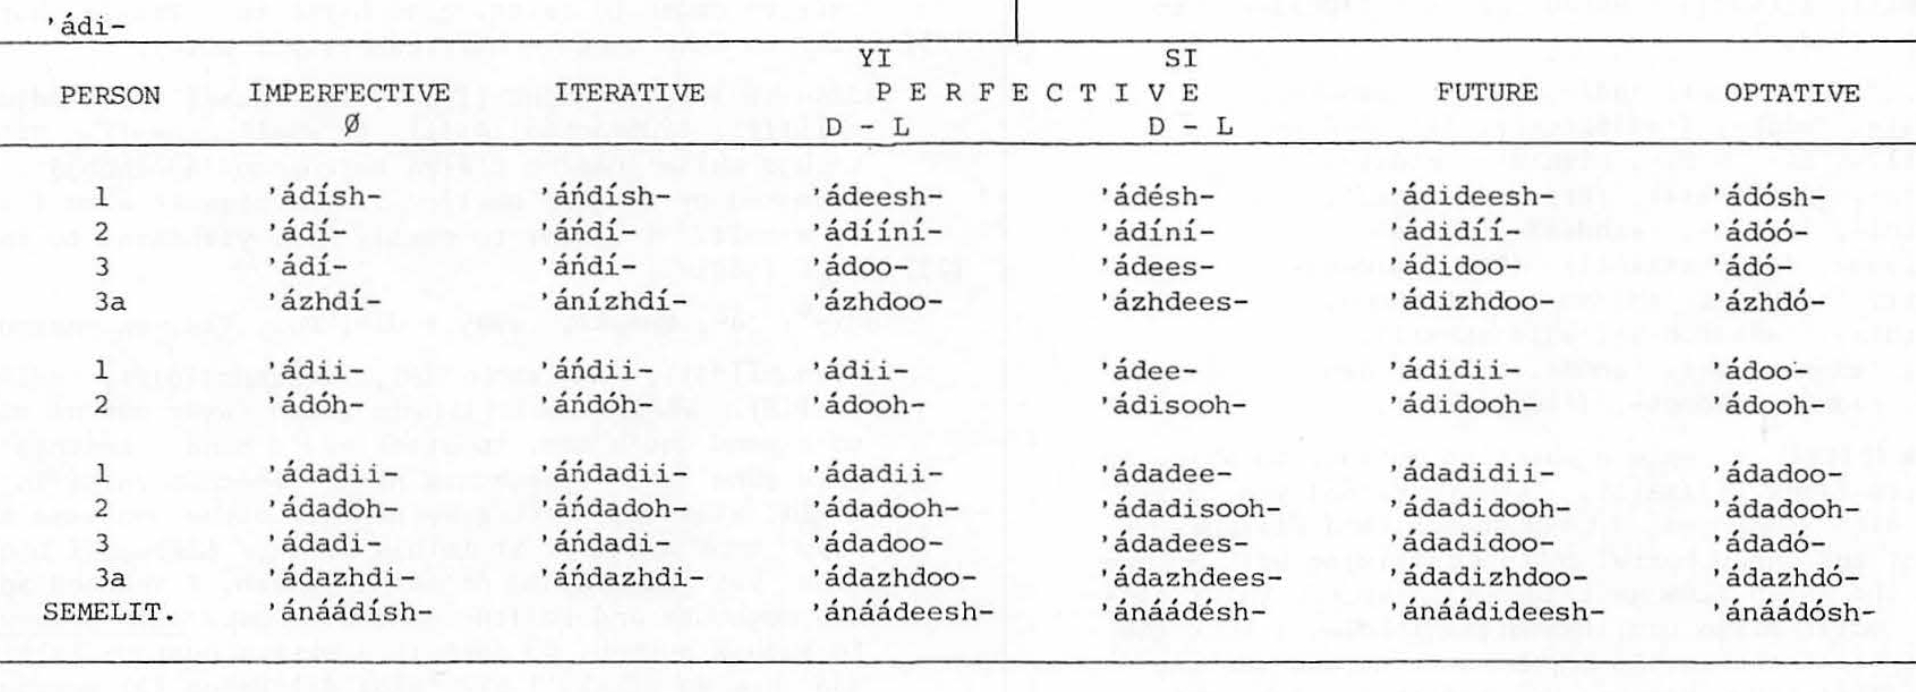
\includegraphics[width=\linewidth]{figures/conjug.jpg}
    \caption{Example of conjugation table for verbs with the prefix string \textit{’ádi-} (\cite[part II:23]{Young:1987uj}).}
    \label{fig:conjug}
\end{figure}

These tables enable users to construct other person/number forms. To form the second-person singular optative of \textit{’ádísk’ąąs}, for instance, one would combine the optative prefix string \textit{’ádóó-} from the table with the stem \textit{k’ąąs}, yielding \textit{’ádóók’ąąs} `you may stretch yourself'. For the Perfective columns, the classifier as well as the conjugation prefixes in Position VII (\textit{si-}, \textit{ni-}, \textit{yi-} or \textit{Ø-}) are necessary to locate the correct form. The perfective form of \textit{’ádisk’ąąs} is \textit{’ádésk’ąąs}, and therefore belongs to the second column of the perfective conjugation, \textit{’ádésh-}, \textit{’ádíní-}, \textit{’adees-} etc. (\textsc{si}-perfective). Phonological processes, such as consonant harmony (changing \textit{’ádésh-} to \textit{’ádés-} before a stem with /s/), must also be applied.

Some entries, like \textit{’ádádiisdzííd} (`I am sipping it'), list their full conjugation paradigm directly if it is not shared by other verbs. The conjugation can be located in an indented part, as shown of the entry of \textit{’ádádiisdzííd} in \figref{fig:adadiisdziid}.

\begin{figure}
    \centering
    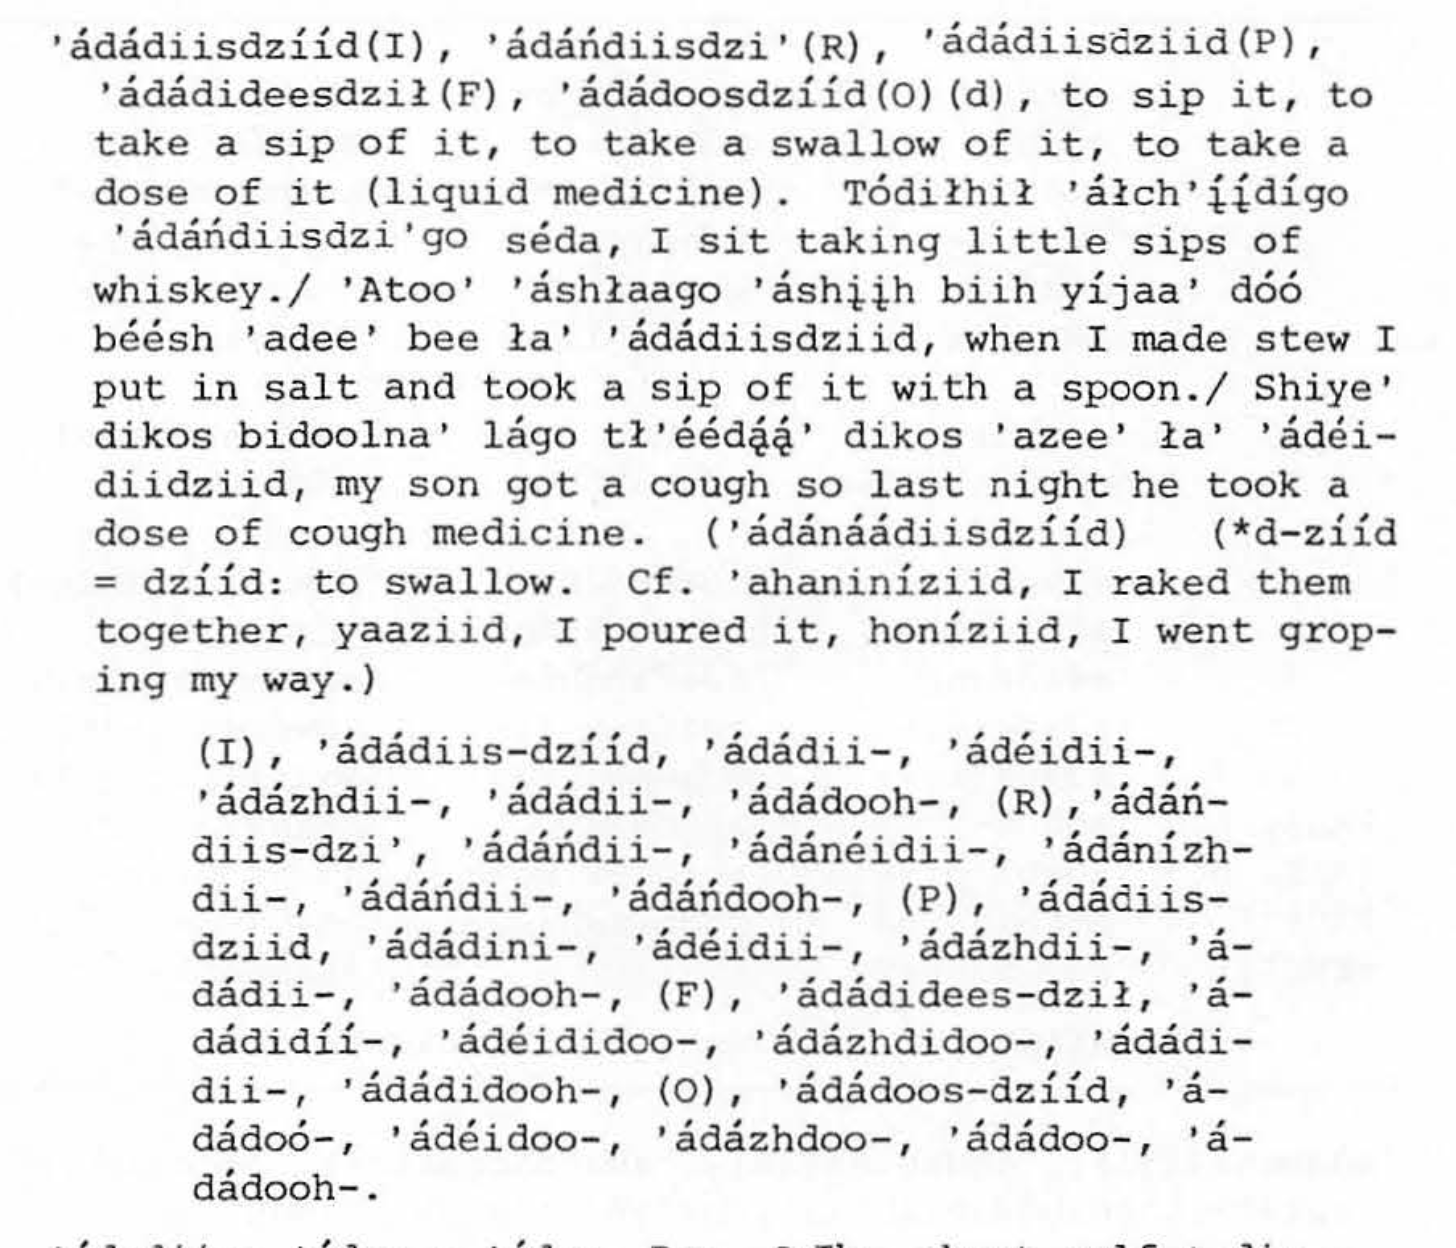
\includegraphics[trim={0 20 0 0},clip,width=\linewidth]{figures/adadiisdziid.png}
    \caption{Example of a verbal entry with its own conjugation in \textit{The Navajo language.} (\cite[7]{Young:1987uj})}
    \label{fig:adadiisdziid}
\end{figure}

The structure of listing verbs in their full form is particularly valuable for working with naturally occurring texts, as it begins with actual word forms. However, for glossing, which requires breaking words into smaller morphological entities, a templatic approach is also necessary.

\subsubsection{Verbal entries in the \textit {Analytical lexicon} (1992)}

The \textit {Analytical lexicon} (\cite{Young:1992bd}) takes a complementary, stem-based approach. Since Navajo verb stems alternate for both inflectional mode and more lexicalized aspectual categories, this organization provides a different analytical perspective. A root entry\footnote{In \citet{Young:1992bd}, the terms ``stem'' and ``root'' are not formally distinguished; both refer to the core lexical morpheme of a verb. However, they employ ``root'' specifically as the dictionary entry that represents the entire set of related inflected and derived stems. This canonical entry is based on the perfective (momentaneous or neuter) stem and is typographically distinguished by capitalization, e.g., ZIID (the root/entry) versus ziid (a specific stem).}, such as ZIID (see \figref{fig:ziid}), shows a complete set of stem alternations across the different modes, but also across multiple aspects (e.g., Momentaneous, Conclusive, Continuative).

\begin{figure}
    \centering
    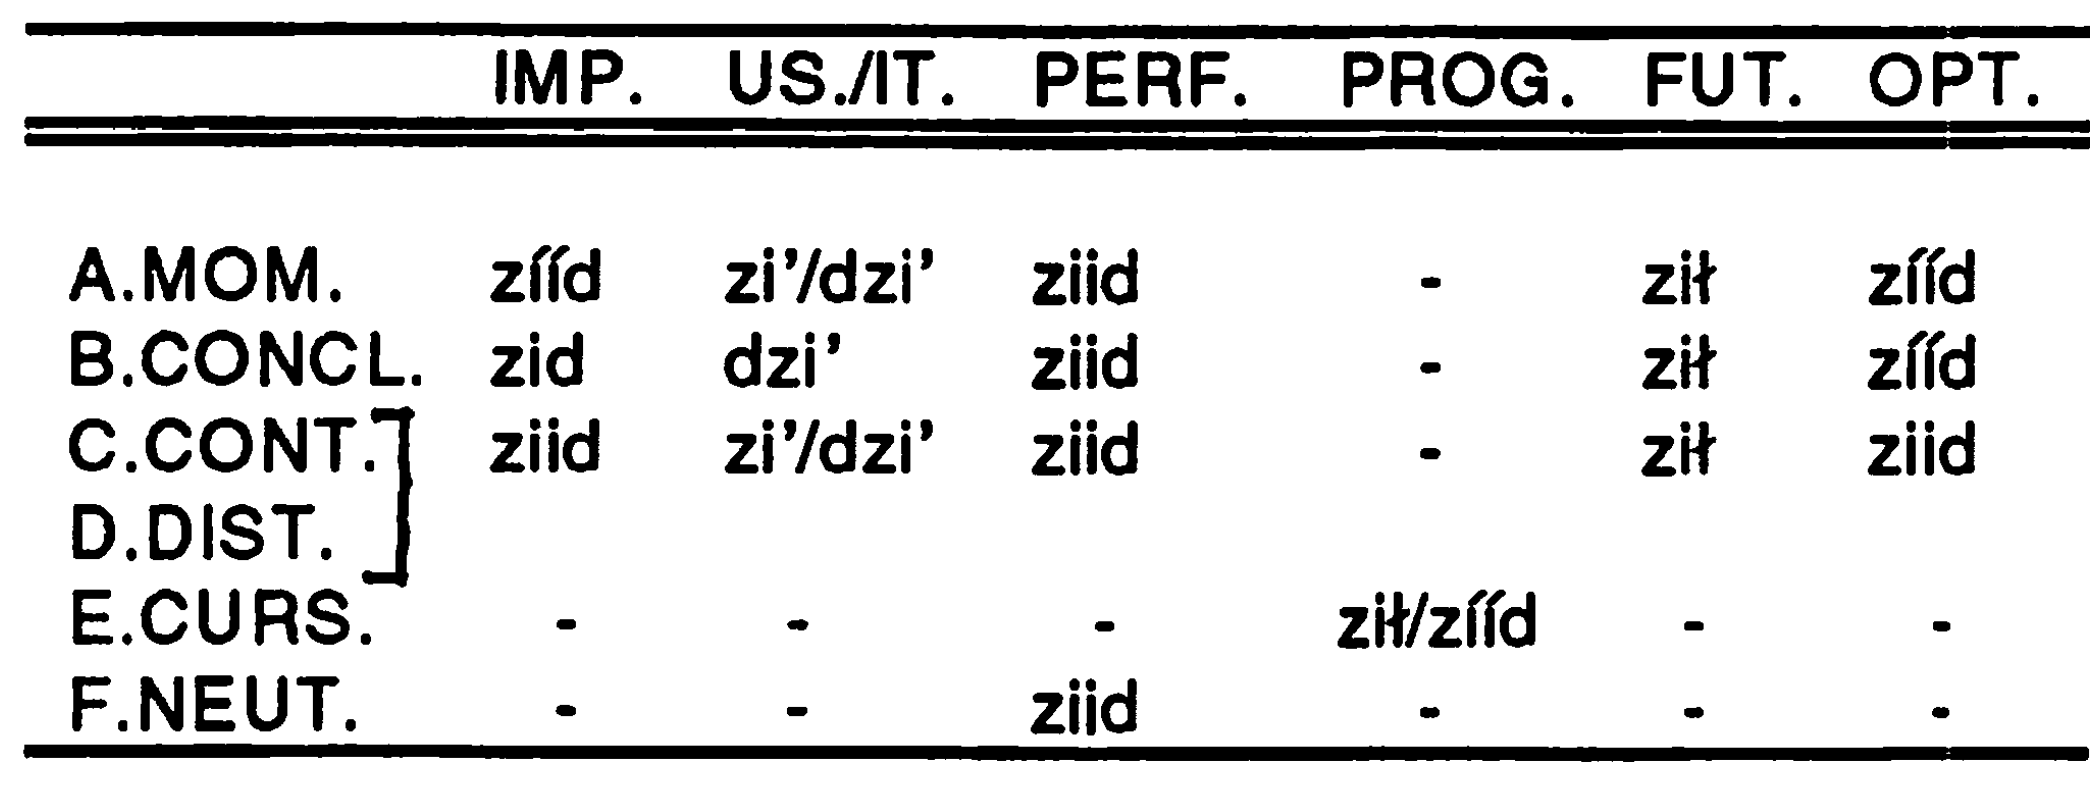
\includegraphics[width=0.7\linewidth]{figures/ziid.png}
    \caption{Stem set of the root ZIID (\cite[749]{Young:1992bd}).}
    \label{fig:ziid}
\end{figure}

Derived verb stems are clustered under one root entry (namely, the stem pertaining to the perfective mode and the momentaneous aspect). Sub-entries specify different aspects, classifiers, and thematic/derivational prefixes, creating distinct verb themes. These themes are cross-referenced to the 1987 dictionary. For example, the verb \textit{’ádádiisdzííd} (\figref{fig:adadiisdziid}) is located under the root ZIID, within the Momentaneous Aspect sub-entry, the D-classifier sub-sub-entry, and the thematic prefix \textit{ádádii-} (see \figref{fig:adadiisdziid-analyt}). Full word forms are reached only after following these analytical steps (Root (ZIID) > Aspect (Momentaneous) > Classifier (D-classifier) > Prefixes (\textit{’ádádii}) > Conjugation prefixes in Position VII (Ø for imperfective and Ø for perfective). However, the entry provides only the imperfective and perfective verb forms. The remaining modes (Iterative, Future, and Optative) are predictable through the conjugation tables in the Appendix or by consulting the corresponding entry in the 1987 dictionary, whose page number (e.g., p. 7) is indicated after the conjugation prefixes (Ø/Ø). This is shown in \figref{fig:adadiisdziid-analyt}.

\begin{figure}
    \centering
    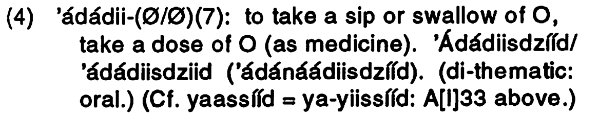
\includegraphics[width=0.7\linewidth]{figures/adadiisdziid-analyt.png}
    \caption{Entry of \textit{ádádiisdzííd} in the \textit{Analytical lexicon} (\cite[750]{Young:1992bd}).}
    \label{fig:adadiisdziid-analyt}
\end{figure}

In contrast, the 1987 volume lists fully inflected forms without analytically separating thematic/derivational prefixes. Consequently, verbs from the same stem but different aspects appear in separate entries. For instance, \textit{bik’éssid} `to pour it over it'; (\figref{fig:bikessid-analyt}) and \textit{’ádádiisdzííd} (\figref{fig:adadiisdziid}) are listed separately in the 1987 dictionary (under ``\textsc{b. conclusive}'' and ``\textsc{a. momentaneous}'' respectively), despite sharing the stem ZIID. In the Analytical Lexicon, they are also listed separately (\figref{fig:bikessid}) but unified under the same stem ZIID which is distinguished by aspect (\textit{’ádádiisdzííd} under Momentaneous, \textit{bik’éssid} under Conclusive).

\begin{figure}
    \centering
    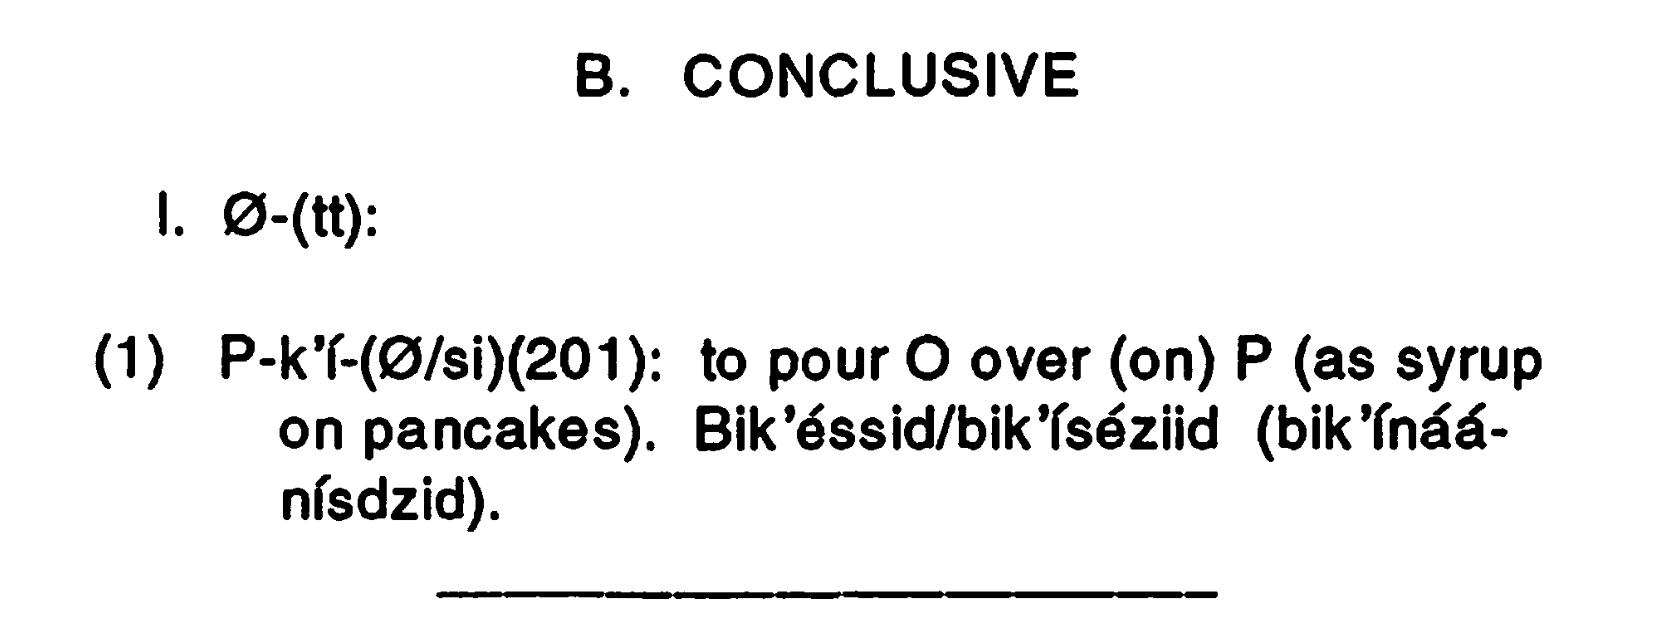
\includegraphics[width=0.7\linewidth]{figures/bikessid-analyt.png}
    \caption{\citet[750]{Young:1992bd} entry of \textit{bik’éssid}.}
    \label{fig:bikessid-analyt}
\end{figure}

\begin{figure}
    \centering
    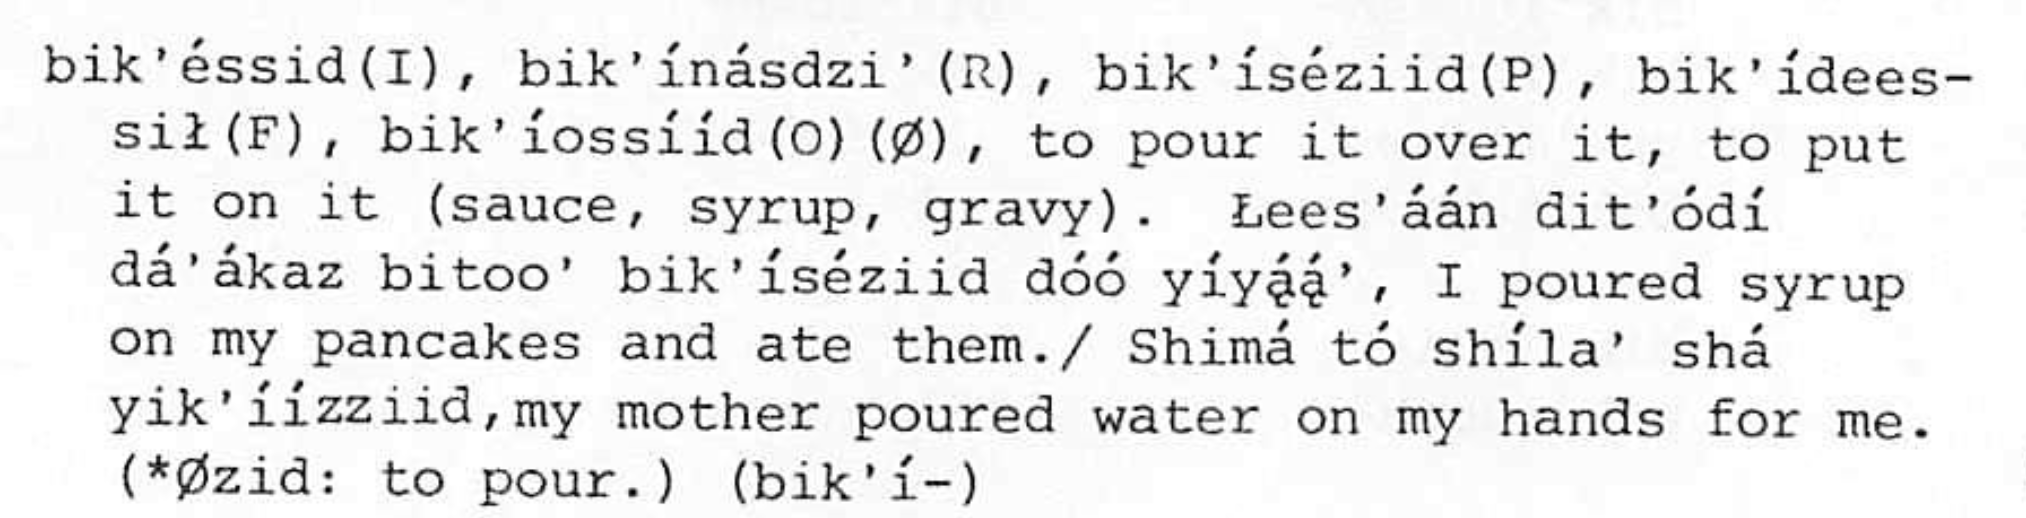
\includegraphics[width=0.7\linewidth]{figures/bikessid.png}
    \caption{\citet[201]{Young:1987uj} entry of \textit{bik’éssid} `to pour it over it'.}
    \label{fig:bikessid}
\end{figure}

The cross-referencing between the two works, where the \textit {Analytical lexicon} provides page numbers to the 1987 dictionary, makes them indispensable companion tools. For this corpus project, both were used extensively. The 1987 volume provided attested word forms and conjugation patterns, while the \textit{Analytical lexicon} supplied crucial information on stems and lexical aspect, which was included in the gloss.

\subsubsection{The bipartite approach (McDonough 1995)}

We have seen that by abandoning the templatic approach to verbs, prefixes are still distinguished from stems, either in a prefix string that is already conjugated (\cite{Young:1987uj}) or a thematic prefix string (\cite{Young:1992bd}). An additional non-templatic analysis is the Bipartite Constituent Model (\cite{McDonough:1995hp}), which is informed by phonological boundaries of surface forms. It proposes that the Navajo verb is built from two core morphological constituents, and a third, outer domain for disjunct clitics. The schema below is adapted from \citet[28]{McDonough:1995hp}:

\begin{center}
    [Disjunct Domain \#  (Agreement) [Inflectional Constit.] [Verb Constit.] ]\textsubscript{Word}
\end{center}

Where:

\begin{itemize}
    \item \textbf{Disjunct Domain:} Clitic-like elements (adverbials, postpositions) attach to the left edge of the core compound. This corresponds to Positions 0-III in the templatic model.
    \item \textbf{Inflectional Constituent:} Contains a portmanteau \textsc{infl} stem (tense/mode{\slash}subject) and qualifier prefixes, with object agreement prefixes added if verbs are transitive. (Positions IV-VIII of the template)
    \item \textbf{Verb Constituent:} Contains the verb stem and classifier prefixes. (Positions IX and X of the template)
\end{itemize}

This model challenges the slot-and-filler template by arguing that phonological evidence points to strong structural boundaries between the two core constituents. Furthermore, grammatical information like tense, mode and subject agreement is fused into single, portmanteau constituents such as the inflectional and verb stem. \citet{McDonough:1995hp} argues for the bipartite model primarily on learnability grounds. She claims the verb structure must be transparent to learners and that morphological information should be recoverable from phonetics and phonology. This morphological and phonological transparency is best communicated when assuming this fundamental distinction between the \textsc{infl} and verb constituent, which aligns with the minimal disyllabic requirement for verbs (see \cite{Speas:1984mo}). The position-class template, in contrast, is an abstract descriptive tool not reflected in lexical patterns or phonological evidence, making it an implausible model for acquisition.

Adopting this learnability perspective, our glossing strategy for the corpus is deliberately surface-oriented. This approach, designed to enhance accessibility for Navajo speakers, is informed both by McDonough's surface-based model and by our adherence to the conventions of the Young and Morgan dictionaries. The rationale for this combined approach is detailed in \sectref{sec:conventions}.

\subsection{Syntax}

The syntax of Navajo does not exhibit many rigid rules or unpredictable behaviors. Navajo is a verb-final language, with agents generally preceding patients; however, the overt expression of both roles in transitive sentences is quite rare. Grammatical relations involving at least one speech act participant (1st or 2nd person) follow a nominative-accusative alignment marked on the verb. In scenarios with only non-speech act participants, object agreement depends on the animacy and topicality of the referents. According to \citet{Willie:2000up}, for third-person referents, entities of higher animacy precede those of lower animacy. Whether higher-ranked entities act on lower-ranked entities or vice versa, i.e., the grammatical roles of agent and patient, is determined by special third-person object agreement on verbs (\textit{yi}- vs. \textit{bi}-, respectively). This is shown in example (\ref{ex:intro2}). Here, `boy' ranks higher than `horse'.

\ea\label{ex:intro2}
    %\textup{Common nouns in A and P roles (\cite[364]{Willie:2000up})}\\
    \ea
    \textit{’Ashkii łį́į́’ yiztał}\\
    \glll \textup{’ashkii} \textup{łį́į́’} \textup{\textbf{yi}-z-tał}\\
	boy horse \textbf{\textsc{3.yi}}-\textsc{3.si.perf}-kick.\textsc{perf}\\
    A P V\\
    \glt `The boy kicked the horse.' %\exsource{overheard conversation}
    \ex
    \textit{’Ashkii łį́į́’ biztał}\\
    \glll \textup{’ashkii} \textup{łį́į́’} \textup{\textbf{bi}-z-tał}\\
    boy horse \textbf{\textsc{3.bi}}-\textsc{3.si.perf}-kick.\textsc{perf}\\
    A P V\\
    \glt `The boy was kicked by the horse.'\exsource{Adapted from \cite[364]{Willie:2000up}}
    \z
\z
    
If the agent and patient rank equally in animacy, the order can be flexible, but topicalized entities always precede those that are focused. For this reason, Navajo is considered a ``Topic-Focus-Verb'' language rather than a ``Subject-Object-Verb'' language.

In addition, Navajo is a pro-drop language. The influential Pronominal Argument Hypothesis (\cite{SandovalJelinek:1989ke}) applied to Navajo (\cite{Speas:1990kf}, \cite{Hale:2006wh}) argues that the verbal agreement prefixes constitute a non-configurational clause, with free nominals as adjuncts. Consequently, the traditional concept of a ``verb phrase'' is not fully applicable to Navajo, as verbs alone can constitute entire clauses. However, \citet{Willie:1995zc} argue for configurationality on the discourse level since the order Topic-Focus-V is consistent. \citet{Hale:2001aq} accounts for configurationality within the verb and posits morphological vP nodes. Beyond the clause, \citet{Hale:1977li} propose phrase structure trees for multiple utterances, showing that while the clausal syntax is flat, there is great complexity within noun phrases, and within verbs. They identify the following phrases: Clause, Noun Phrase, Postpositional Phrase, Enclitic Phrase. 

A noun phrase consists of a noun or pronoun, with additional modifiers that may precede or follow the head noun. Property concepts that modify nouns follow the noun, and since many derive from verbal expressions, the category of ``adjective'' is also not clearly applicable. In noun phrases, possessor nouns precede possessed nouns, and the possessed noun carries a prefix that agrees in person and number with the possessor. A complex noun phrase exhibiting a deverbal noun with multiple modifiers is given in (\ref{ex:intro3}).

\ea\label{ex:intro3}
    %\textup{Complex noun phrase (modified from Tony Tsosie 12.2)}\\
    \textit{Díí chidí naat’a’í ’ayóí ’ádaniłtsxooígíí bitsiits’iin}\\
    \glll \textup{díí} \textup{chidí} \textup{naa-t’a’=í} \textup{’ayóí} \textup{’á-da-ni-ł-tsxoo=ígíí} \textup{bi-tsiits’iin}\\
	this car \textsc{cont}-fly.\textsc{impf}.\textsc{cont}=\textsc{nmlz} very	\textsc{th}-\textsc{distr}-\textsc{th}-\textsc{ł}-be.very.big.\textsc{neu}.\textsc{impf}=\textsc{pres}.\textsc{ref} 3.\textsc{poss}-head\\
    demonstrative noun {deverbal\_noun (possessor)} adverb {deverbal\_adjective} {possessed\_noun}\\
    \glt `These big planes' motors.' \exsource{modified from Text I: \ref{ex:text9-12-2}}
\z

This structure is mirrored in postpositional phrases, where the modified noun follows the postposition, which similarly displays a prefix that agrees in person and number with that noun. Postpositions, however, can also act as adverbs or even be incorporated into the verb, inheriting the agreement prefix.

\ea\label{ex:intro4}
    %\textup{Postpositions (NCHN; TRR1: 36.1)}\\
    \textit{beeldléí yee ’ákászaazgo}\\
    \glll \textup{beeldléí} \textup{y-ee} \textup{’á-ká-s-zaaz=go}\\
    blanket 3.\textsc{yi}.\textsc{poss}-with \textsc{refl}.\textsc{poss}-on-3.\textsc{si}.\textsc{perf}-belt.\textsc{neu}.\textsc{perf}=\textsc{sub}\\
    %blanket {with it} {belted around himself}\\
    noun postposition postposition-verb\\
    \glt `blanket wrapped around his middle.' (lit. `with the blanket it is belted around himself.') \exsource{Text A: \ref{ex:text1-36-1}}
\z

Because the prefixes on possessed nouns and postpositions are identical to object prefixes in verbs, nouns, postpositions and verbs are morphologically connected, which blurs the distinction between different parts of speech. Additionally, enclitics may attach to any of these word classes or phrases. In terms of negation, Navajo employs a preverbal negative marker, often coupled with a second marker at the end of the sentence, creating a bipartite negation structure:

\ea\label{ex:intro5}
    %\textup{Negation (NCHN; CT:2.2)}\\
    \textit{’Éí bízhi’ígíí dóó shash jiníi da}\\
    \gll \textup{’Éí} \textup{bí-zhi’=ígíí} \textup{doo} \textup{shash} \textup{ji-níi} \textup{da}\\
	That	3.\textsc{bi}.\textsc{poss}-name=\textsc{pres.ref} not bear \textsc{anim}-say.\textsc{neu}.\textsc{impf}	not\\
    \glt `One does not mention their name ``bear''.' \exsource{Text F: \ref{ex:text6-2-2}}
\z

\section{Glossing approach in the Navajo Corpus of Historical Narratives}\label{sec:conventions}

Throughout the scholarly tradition of Navajo and Athabaskan languages, linguists have typically avoided exhaustive segmentation, focusing only on categories pertinent to the specific discussion (\cite{Denk:2024aq}; \cite{Hargus:2020wv}). This prioritizes practicality, often simplifying glosses to the word level or omitting morphological detail due to space constraints and audience needs. For instance, the Navajo Conversational Corpus (\cite{Mithun:2009nl}) provides only free translations, and even \citet{Young:1987uj} refrain from full morphemic glossing in narrative examples. As mentioned previously, the central analytical challenge is the morphological structure itself, where lexical, derivational, and inflectional information is spread across verb positions, making a consistent morpheme-based approach inherently difficult.

To address this, \citet{Denk:2025zp} developed a glossing strategy for the Navajo Corpus of Historical Narratives (NCHN) that balances linear analysis with faithfulness to surface structure. The corpus implements this through several annotation tiers:

\begin{itemize}
    \item \textbf{Word:} Presents Navajo words as they appear in the narrative, with minimal corrections for typographical errors.
    \item \textbf{Morpheme:} Displays morphemes in their surface forms (morphs), segmented with hyphens for affixes and equal signs for clitics.
    \item \textbf{Lexical Entry:} Represents the underlying forms of morphemes, with one form chosen as the headword, often based on its first occurrence in the corpus.
    \item \textbf{Lexical Gloss:} Provides grammatical information and English translations following the Leipzig Glossing Rules.
    \item \textbf{Lexical Grammatical Information:} Specifies word-class information for stems and affixes (e.g., verbal stem (v), preverbs (PRVB), postpositions (post)).
    \item \textbf{Word Gloss:} Gives an English gloss for the entire word, capturing its compositional meaning.
    \item \textbf{Free Translation:} Provides a sentence-level English translation, typically retaining the original from the source narratives, unless it has been revised for the sake of clarity; in such cases, this is indicated in square brackets.
\end{itemize}

An example of glossing is given below (the Free Translation tier is omitted as this is a single word):

\begin{table}
    \begin{tabular}{llllll}
        \multicolumn{6}{l}{from NCHN (A Childhood Tale; John C. Claw; 13.26)}\\
        Word: & \multicolumn{5}{l}{ndahaazbą́ą́z}\\
        Morphemes: & n- & da- & haa- & z- & bą́ą́z\\
        Lex. Entries: & ni-\textsubscript{5} & da-\textsubscript{3} & h-\textsubscript{1} & si-\textsubscript{1} & bą́ą́z\\  
        Lex. Gloss: & \textsc{th} & \textsc{distr} & \textsc{ser} & 3.\textsc{si}.\textsc{perf} & roll.\textsc{perf}\\
        Lex. Gr. Info: & v:PRVB & Att. to any cat. & v:QUAL & v:AMS & v\\
        Word Gloss: & \multicolumn{5}{l}{they rolled it one after another up to a point}\\
    \end{tabular}   
\end{table}

As shown, the word \textit{ndahaazbą́ą́z} is linearly segmented and glossed, and abandons distributional or holistic word glosses. Consequently, Young and Morgan's templatic positions became a valuable tool for linearly assigning morphemes. However, we also oriented the linear analysis to the surface structure, similar to McDonough's (\citeyear{McDonough:1995hp}) bipartite approach, and abandoned numerical positions. Instead, we clustered morphs from the \textit{Lexical Gloss} tier into functionally defined categories of the \textit{Lexical Grammatical Information} tier. These categories align with the template but involve different clustering, as shown in \figref{fig:verbtemplate}.

\begin{figure}
    \centering
    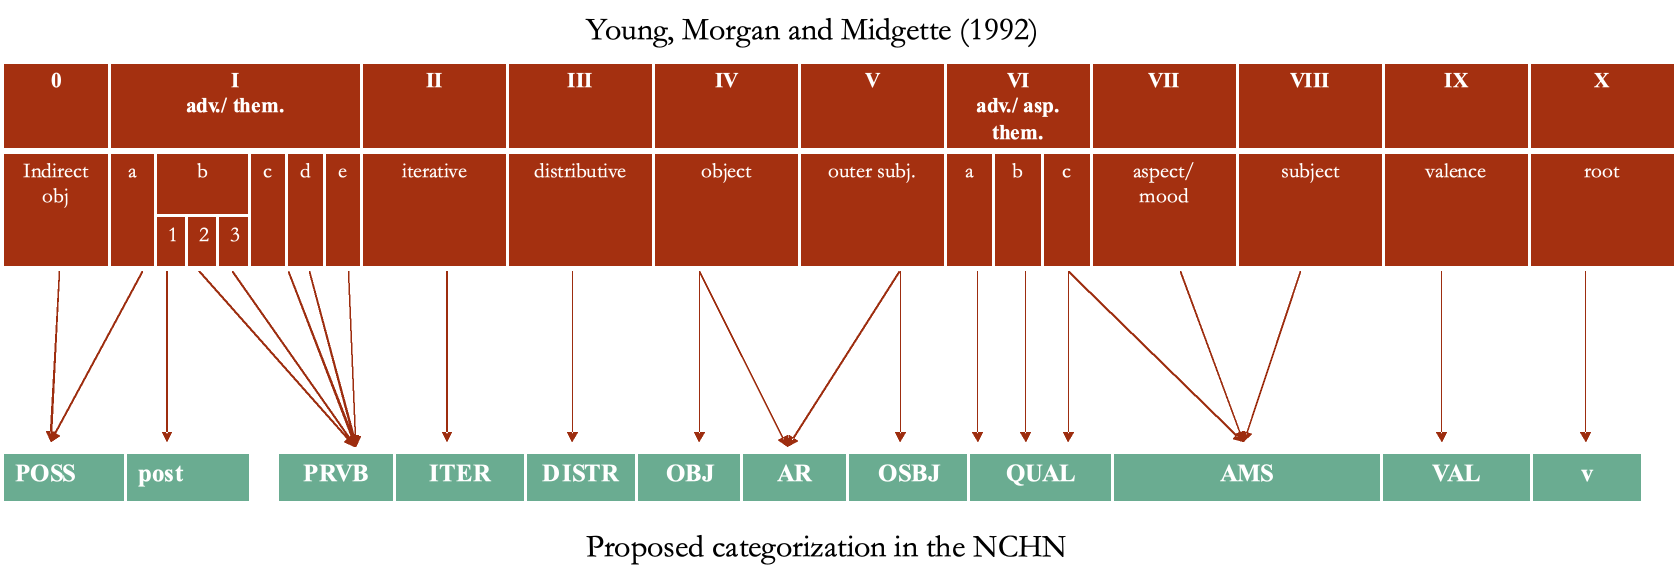
\includegraphics[width=\linewidth]{figures/template.png}
    \caption{Categorization of morpheme positions from \citet{Young:1992bd} in the NCHN (Figure from \cite{Denk:2024aq}). Abbreviations are further explained in the Appendix.}\label{fig:verbtemplate}
\end{figure}

The glossing strategy is governed by three underlying principles:

\begin{enumerate}
    \item \textbf{Surface Faithfulness:} \textit{Do not change the shape of morphs while segmenting.}
    
    Morphemes are segmented in their surface form. For example, \textit{ndahaazbą́ą́z} is segmented as \textit{n-da-haa-z-bą́ą́z}. Variant forms like the seriative \textit{haa-} are registered as allomorphs of a single lexical entry (e.g., h-), with the first corpus instance typically chosen as the headword. In an approach that adopted the Young and Morgan template strictly, this word would be segmented as ni\textsuperscript{I}-da\textsuperscript{III}-hi\textsuperscript{VI}-siV\textsuperscript{II}-Ø\textsuperscript{VIII}-Ø\textsuperscript{IX}-bą́ą́z\textsuperscript{X} (with numbers of positions in superscript).
    \item \textbf{Category Faithfulness:} \textit{Keep number of categories and morphs in a manageable range, and do not merge or split them.}

    This principle streamlines annotation by consolidating morpheme categories to a manageable set, reducing redundancy while ensuring consistent assignment. It overrides exhaustive segmentation where fusion is systematic. For instance, the diverse thematic and adverbial morphemes from positions Ib(2,3)-e in Young and Morgan's template are grouped as a single Preverb (PRVB) category. This grouping of similar categories also applies to postpositions, where freestanding and verb-incorporated forms are glossed identically, as in the following example:\footnote{One difference between the glossed text presented in this volume and the corpus is that incorporated postpositions are still hyphen-segmented here, whereas in the corpus they are treated as stems. Without the hyphen, two morphemes such as \textit {ká} and \textit{s-} would be conflated as \textit{kás-} in the current text, whereas with the hyphen they appear as \textit{ká-s-}. In FLEx, by contrast, the separation is maintained through spaces and multiple tiers of annotation -- a level of detail this volume does not display. Instead of splitting up one word into two words, this approach preserves the integrity of the word as it appears in the original text.}

\begin{table}
    \begin{tabular}{lp{1,1cm}lllp{1,1cm}ll}
        \multicolumn{8}{l}{from NCHN (The Trouble at Round Rock; Mexican Clansman; 36.1)}\\
        beeldléí&\multicolumn{2}{l}{\textbf{yee}}&\multicolumn{5}{l}{\textbf{’áká}szaazgo}\\
        beeldléí&\textbf{y-}&\textbf{ee}&\textbf{’á-}&\textbf{ká}&s-&zaaz&=go\\
        beeldléí&y-\textsubscript{1}&ee&’á-\textsubscript{3}&káá’\textsubscript{1}&si-\textsubscript{1}&zaaz\textsubscript{1}&=go\\
        blanket&3.\textsc{yi}.\textsc{poss}&with&\textsc{refl}.\textsc{poss}&on&3.\textsc{si}.\textsc{perf}&belt.\textsc{neu}.\textsc{perf}&=\textsc{sub}\\
        n&any cat.&\textbf{post}&any cat.&\textbf{post}&v:AMS&v&prt\\
        blanket&with it&&\multicolumn{5}{l}{belted around himself}\\
        \multicolumn{8}{l}{blanket wrapped around his middle}\\
    \end{tabular}   
\end{table}

    Similarly, aspect, mood, and subject markers (from Young and Morgan's positions VIc, VII, and VIII) are fused into a single Aspect-Mood-Subject (AMS) category (aspect, mood, and subject) because they often merge into unsegmentable portmanteau morphs (e.g., \textit{s-} for 3.\textsc{si}.\textsc{perf}). This grouping, acknowledging the fusional nature of this domain as suggested by McDonough's (\citeyear{McDonough:1995hp}) bipartite model, facilitates annotation and retrieval. An example of two consolidated positions is the category of the Areal (AR). These two subject and object uses of the prefix \textit{ha-}/\textit{ho-}/\textit{h-} do not co-occur, and therefore, this prefix has been assigned a single category. Similarly, paradigms that share structural features, like the usitative/imperfective or future/progressive within the AMS category, are glossed as one (imperfective and progressive, respectively).

    \item \textbf{Form-Meaning Exhaustion:} \textit{Segment as much as possible and assign as much meaning as possible to segmented parts.}

    Words are segmented down to single morphs, but not below the surface level. This can lead to what would be a single category in a distributed/holistic approach being annotated in multiple tiers. A clear example is the future paradigm: forms like \textit{díí}- (2\textsc{sg}.\textsc{fut}) are segmented as \textit{d-íí} and glossed as \textsc{fut}-2.\textsc{sg}.\textsc{prog}. This reflects its structural composition from a future marker plus the progressive paradigm as seen in Table 5.

    \begin{table}
        \caption{Future paradigm compared to progressive paradigm (\cite[907,910]{Young:1992bd}). The letter C denotes any thematic consonant preceding the morpheme sequence.}
        \label{tab:placeholder}
        \begin{tabularx}{.6\linewidth}{XXX}
            \lsptoprule
            &\textsc{future}&\textsc{progressive}\\
            \midrule
            1\textsc{sg}&\textit{deesh}-&\textit{Ceesh}-\\
            2\textsc{sg}&\textit{díí}-&\textit{Cíí}-\\
            3&\textit{doo}-&\textit{Coo}-\\
            1\textsc{du}/\textsc{pl}&\textit{dii(d)}-&\textit{Cii(d)}-\\
            2\textsc{du}/\textsc{pl}&\textit{doo(h)}&\textit{Coo(h)}-\\
            \lspbottomrule
        \end{tabularx}
    \end{table}

    This grouping, again, avoids the need for a separate, fully inflected future paradigm (aligning with Category Faithfulness). In addition, a similar principle is used for verb stems, which are glossed for specific sub-aspects (e.g., \textsc{neu}.\textsc{impf}) based on the stem tables in \citet{Young:1992bd}.

\end{enumerate}

In summary, we annotated words according to a linear analysis that oriented itself on the template but included as much grammatical information as possible, resulting in multiple annotation of categories in verbs, without over-exhausting the number of categories. Thus, different from Young and Morgan's analyses of verbs (fully conjugated vs. verb themes), we retained linearity in segmenting the verbs but glossed some the segmented morphs according to categories that might be otherwise considered distributed (such as Continuative, which we glossed for the prefix and the stem). These principles resulted in a practical, user-friendly annotation system that aligns with the template of Young and Morgan while simplifying the relationship between morpheme form and category.

This entire consideration of morpheme glossing and the multiple tiers that we applied to the corpus are essential to understanding the segmentation and glossing in this publication for Open Text Collections, even when more technical tiers like \textit{Lexical Entry} and \textit{Lexical Grammatical Information} are omitted. We acknowledge that the glossing of Navajo and other Dene languages is a controversial issue, not only culturally but technically (\cite{Hargus:2020wv}; \cite{Denk:2024aq}). Nevertheless, we opted for the continuation of the linear approach that we have developed in the corpus because we think that the glossing tier \textit{Lexical Gloss} best captures the categories that a reader is interested in, whether they believe Navajo's categories are templatic or distributed. Readers are encouraged to read the Corpus Guidelines on the webpage of the corpus (\url{https://digitalrepository.unm.edu/navajocorpus/1/}) to get a better understanding of the different glossing conventions.

\section{Provenance}

This publication presents texts from the March 2025 version of the morphologically annotated Navajo Corpus of Historical Narratives (\cite{Denk:2025zp}). The corpus contains Navajo texts that were originally selected, transcribed, and published by Robert W. Young and William Morgan, two foundational figures in Navajo linguistic documentation. The texts come from two collections: \textit{The trouble at Round Rock} (\citeyear{Young:1952cy}) and \textit{Navajo historical selections} (\citeyear{Young:1954jz}), each published by the U.S. Bureau of Indian Affairs. Their works focused on documenting and preserving narratives relevant to Navajo history, culture, and language, as well as introducing accessible Navajo language texts to broader audiences. The Navajo Corpus of Historical Narratives expands on their legacy by providing annotated translations that allow for more detailed linguistic analysis. 
Any additions, changes, or omissions in the free translation are indicated by square brackets in the corpus, and these markings are retained in the ``English translation'' section for each text in this volume.

\subsection{Ethics}

This publication ensures respect for the rights of all contributors and the communities whose narratives and linguistic data are represented. The historical narratives analyzed in this work ultimately originate from Navajo authors from the late 19\textsuperscript{th} and early 20\textsuperscript{th} centuries and have therefore a primary connection to the Navajo community. Through the scholarship of \textit{’Ádahooniłígíí} and Young and Morgan, these texts have been made available to broader audiences. The ethical considerations of that time are not clear.

To ensure compliance with copyright and permissions, due diligence has been conducted regarding the legal status of these materials. Correspondence with relevant administrative bodies, including the Indian Bureau of Education, has indicated that these works are in the public domain, and additional confirmation has been sought from the U.S. Copyright Office to ensure the publication's adherence to copyright regulations. Given these findings, the decision has been made to publish this work as an open-access resource, to ensure accessibility and scholarly integrity.

\subsection{Young and Morgan's historical selections}

The selected narratives from \citet{Young:1952cy,Young:1954jz} offer perspectives on historical events and daily life at the end of the 19th century. Texts from \textit{The trouble at Round Rock} (\citeyear{Young:1952cy}) focus on a specific historical incident, namely a dispute involving Agent Shipley and Black Horse, set against the social and economic backdrop of the Navajo Nation. The narratives from \textit{Navajo historical selections} (\citeyear{Young:1954jz}) cover a broader range of topics, including traditional stories and individual experiences that contribute to a more nuanced understanding of Navajo life and worldview. The narratives chosen for this corpus reflect our intention to represent a broad number of topics that could serve as a basis for studying different narrative styles.

\subsection{Selection criteria}

The selection process focused on ensuring diverse representation across different themes and perspectives within the Navajo community. From \textit{The trouble at Round Rock}, all relevant texts were included to provide a complete view of the central historical incident described. For \textit{Navajo historical selections}, texts were chosen to represent each part of the thematic volume, focusing on narratives that include traditional stories, social commentary, personal anecdotes, and historical insights. This includes different narrative styles, such as first- and third-person perspectives.

\subsection{Selected texts}

A total of 9 texts were selected from the two volumes. Texts \ref{chapter:text01}-\ref{chapter:text03} are from \textit{The trouble at Round Rock}, and Texts \ref{chapter:text04}-\ref{chapter:text09} from \textit{Navajo historical selections}.

\begin{table}
    \caption{The texts in this collection.} \label{tab:texts}
\begin{tabularx}{\textwidth}{llQr}

    \lsptoprule
        \textsc{text} & \textsc{title} & \textsc{author}&\textsc{words}\\
    \midrule

		\ref{chapter:text01}&\textit{The trouble at Round Rock} & Left-Handed Mexican Clansman &2,820\\
        \ref{chapter:text02}&\textit{The trouble at Round Rock} & Howard Gorman &787\\
        \ref{chapter:text03}&\textit{The trouble at Round Rock} & The Nephew of Former Big Man&722\\
        %\midrule
        \ref{chapter:text04}&\textit{The traditional Navajo country} (part I)&no author specified&1,049\\
        \ref{chapter:text05}&\textit{The first mother-in-law} (part I)&Tony Tsosie&640\\
        \ref{chapter:text06}&\textit{A childhood tale} (part II)&John C. Claw&2,036\\
        \ref{chapter:text07}&\textit{Our abuse} (part III)&Dan Phillips&1,268\\
        \ref{chapter:text08}&\textit{The special grazing regulation} (part III)&The Blind Man's Daughter&258\\
        \ref{chapter:text09}&\textit{I flew over Navajo land} (part IV)&Tim Yazzie&1,194\\
    \midrule    
        \textbf{Total}&&&\textbf{10,774}\\
    \lspbottomrule
    \end{tabularx}
\end{table}

\section{Genres, styles and main themes}

The genres within the corpus range from historical accounts and adventure tales to traditional narratives and personal recollections. Narrative styles vary accordingly, with some texts taking on formal, descriptive tones, while others exhibit conversational or introspective qualities. The variation in genres and narrative voices provides a broad spectrum of discursive forms, including dialogue, descriptive passages, and self-reflective commentary. The corpus thus promotes, if limited, a diverse representation of themes from the larger pool of narratives, and is a valuable resource for studying Navajo grammar, stylistics, and narrative construction, as well as for understanding the cultural contexts in which these narratives are embedded. The main themes of the narratives are discussed in \sectref{sec:themes}.

\section{Speakers/narrators}

As listed above, the narrators include both named individuals and anonymous voices. Texts in \textit{The trouble at Round Rock} feature historical figures recounting first-hand experiences, while selections from \textit{Navajo historical selections} highlight a range of storytellers, including John C. Claw and Tony Tsosie, who bring personal history and traditional knowledge to life. In addition, it is worth mentioning that traditional knowledge, even if kept distinct from individual tales, exhibits the diversity of families passing these stories to their offspring and therefore also personal accounts and interpretations. As such, the autorship of traditional stories includes an entire chain of past narrators.

\section{Main themes}\label{sec:themes}

The texts enumerated story above in \tabref{tab:texts}, exhibit the following main themes, portrayed in \tabref{tab:themes}.

\begin{table}[]
    \caption{Distribution of main themes across the narratives}
    \label{tab:themes}
    \begin{tabularx}{.85\textwidth}{Xlllllllll}
        \lsptoprule
        \textsc{main themes}&\ref{chapter:text01}&\ref{chapter:text02}&\ref{chapter:text03}&\ref{chapter:text04}&\ref{chapter:text05}&\ref{chapter:text06}&\ref{chapter:text07}&\ref{chapter:text08}&\ref{chapter:text09}\\
        \midrule
        \textsc{historical events}&\times&\times&\times&&&&\times&\times&\times\\
        \textsc{politics}&\times&\times&\times&&&&\times&\times&\\
        \textsc{individual experience}&\times&&&&&\times&\times&\times&\times\\
        \textsc{adventure}&&&&&&\times&&&\times\\
        \textsc{traditional knowledge}&&&&\times&\times&\times&&&\\
        \lspbottomrule
    \end{tabularx}
\end{table}

The main themes are well distributed across the corpus, focusing on experiences on the individual and collective level. In the following, these themes will be commented on in relation to the texts.

\subsection{Historical events and politics}

\textit{The trouble at Round Rock} versions (Texts \ref{chapter:text01}, \ref{chapter:text02}, \ref{chapter:text03}) focus on historical events and political tensions affecting the Navajo people during the late 19th century. The core of these stories revolves around the conflict between Agent Shipley and Black Horse, which instantiates broader socio-political struggles and the tensions arising from U.S. government encroachment. These narratives not only recount specific incidents but also show the effects of imposed policies on the Navajo way of life and governance. They highlight clan leaders and influential community members who are forced to act due to external pressures, providing a Navajo account on the political resistance.

The \textit{Navajo historical selections} volume offers additional political commentary, notably in \textit{Our abuse} (\textref{chapter:text07}) and \textit{The special grazing regulation} (\textref{chapter:text08}). These narratives focus less on the unfolding of historical events but instead more on government-imposed regulations and their consequences for Navajo lands and livelihoods at the time of narration. Dan Phillips, for instance, describes the hardships and frustrations of the Navajo community as they faced restrictive grazing regulations, which drastically altered traditional livestock practices. These stories account for the ongoing tension between Navajo self-governance and federal oversight, tying back to earlier conflicts like \textit{The trouble at Round Rock}. Finally, Tim Yazzie's account on his flight over the Navajo Nation to deliver aid (\textref{chapter:text09}) relates to the historical ``Blizzard of 1949'' and intersects with the livestock reduction policies.

\subsection{Individual experiences and adventures}

Individual adventures are recounted in many of these narratives and provide personal perspectives on broader historical themes. For instance, \textit{A childhood tale} by John C. Claw (\textref{chapter:text06}) describes formative events and challenges faced by the narrator during his early years and highlights how historical events intersected with personal development. Similarly, \textit{I flew over Navajo land} by Tim Yazzie (\textref{chapter:text09}) offers a more immediate account of adventure and the dangers of being on a plane mission. Yazzie's narrative stands out for its sense of freedom and exploration, as he describes the landscapes and people he encountered from an airplane, providing an almost ethereal view of his homeland. These personal reflections lend an intimate tone to what is also a historical event, namely the severe Blizzard of 1949. Furthermore, the stories \textit{Our abuse} (\textref{chapter:text05}) and \textit{The special grazing regulation} (\textref{chapter:text08}) provide individual insights into the hardships faced during the Livestock Reduction Policies. Lastly, the first version of \textit{The trouble at Round Rock} (\textref{chapter:text01}) can also be regarded as an individual experience, since Left-Handed Mexican Clansman was present during the fight between Black Horse and Agent Shipley.

\subsection{Traditional knowledge}

In \textit{The traditional Navajo country} (\textref{chapter:text04}), the anonymous narrator explores the Navajo connection to their land and emphasizes the cultural and spiritual significance of the geography around them. This piece promotes traditional knowledge, as the narrator details the mountains, plants, and animals with reverence and precision. By narrating the symbolic meaning and traditional uses of different elements in the environment, this text helps understand Navajo cosmology and the land as a source of identity and wisdom.
	
Similarly, \textit{The first mother-in-law} narrative (\textref{chapter:text05}) emphasizes traditional customs, such as family roles, marriage, and respect for elders and deities. These stories are not only informative but also preserve the cultural practices and beliefs that define Navajo social life. Tony Tsosie's perspective sheds light on the dynamics of family relations and their societal expectations. Also, John C. Claw's childhood story (\textref{chapter:text06}) incorporates elements like taboos which can be counted as part of the traditional narrative inventory.

Having established the main themes of the collection, the focus now turns to the primary sources themselves. Part \ref{part:texts}, allows these works to speak for themselves, giving the reader direct access to their voices and stories in full detail.
